\chapter{Testing}
\label{ch:testing}

\section{Overview}

This chapter describes the implementation of the \ref{ch:methodology} chapter's methodology through the usage and analysis of a data set provided by Arcos \cite{arcos}. The results obtained in the various steps of the methodology are discussed in depth and the results are analyzed trying to highlight the most noticeable anomalies.

The chapter \ref{sec:testing-dataset} introduces the AIS source data used for this testing session. Their numbers and properties are described. In addition, the DBSCAN results are described numerically as the number of clusters and outliers resulted from the implemetnation.

A graphical representation of the clusters resulting from running the DBSCAN with these data is illustrated in the chapter \ref{sec:pca}.

In the chapter \ref{sec:testing-importance}, a classification of the features that most contributed to the outliers being considered as such is provided, their properties such as model accuracy and T-test value are evaluated in order to select the three most important features.

In the chapters \ref{sec:anomaly-1}, \ref{sec:anomaly-2}, \ref{sec:anomaly-3} the three resulting outliers are described in detail, and an attempt is also made to give an in-depth interpretation of them.

\clearpage
\subsection{The original Dataset and clustering results}
\label{sec:testing-dataset}
The source dataset selected to carry out testing of the described methodology is as mentioned composed of AIS messages.
Nel dettaglio, si tratta di messaggi provenienti da navi che hanno attraversato la zona artica e dintorni negli anni 2019, 2020 e 2021.
In numbers:
\begin{itemize}
\item 95,294,750 AIS messages;
\item 10,058 different vessels;
\item 6,777 segments (trips) generated.
\end{itemize}

I dati in questione hanno attraversato tutti gli step descritti nel capitolo \ref{ch:methodology}, dal data cleaning fino all'implementazione del DBSCAN.

Attraverso un processo di hyperparameter tuning, come descritto nella sezione \ref{sec:tuning}, sono stati scelti i parametri di input di DBSCAN 

\begin{center} 
    $\varepsilon$ = 0.8 \, \textit{min\_points} = 5
\end{center} 

Qui segue un dettaglio della dimensione di ogni cluster:
\begin{itemize}
\item Cluster \textbf{\#1}: 4106 trips
\item Cluster \textbf{\#2}: 1178 trips
\item Cluster \textbf{\#3}: 651 trips
\item Cluster \textbf{\#4}: 456 trips
\item Cluster \textbf{\#5}: 230 trips
\item 156 outliers
\end{itemize}

As we can see, the first cluster is significantly larger than the others and represents the travel cluster with features in the most common ranges. Some features with less common values contributed to the other clusters. Instead, trips with values too different from those in the clusters fall into the resulting \textbf{156} outliers.

This resulted in \textbf{5} clusters and \textbf{156} outliers (representing 2.3\% of the number of starting trips). The complete clustering results can be found in the appendix \ref{app:testing-results}.

\clearpage

\subsection{PCA, a graphical clusters representation technique}
\label{sec:pca}

In order to a get an idea of the clusters from a graphical point of view, a \textbf{dimensionality reduction} procedure was used: \textbf{Principal Component Analysis}.
PCA has the task of reducing an input space with n dimensions into a space with smaller number of dimensions.
Since the goal in this case was to obtain a graphical representation of the clusters, the number of components to which the 7 input components were reduced was \textbf{2}.

What DBSCAN produces in this context is a dataset of clusters and all the possible information to locate in a 7-dimensional space (the 7 chosen features, indeed) the trips that were given to it as input.
More precisely, each pathway is classified as:
\begin{itemize}
\item \textbf{Core Point} if it is a point that contributed to the cluster expansion, as described in the section; \ref{subsec:dbscan-example}
\item \textbf{Non-Core Point} if it is a point that has not contributed to cluster expansion;
\item \textbf{Outlier} if for some reason the algorithm did not include the trip in any generated cluster.
\end{itemize}

Of course, it is very complicated to depict a space with a number of dimensions greater than 2, so the result of this DBSCAN would be difficult to represent.

Using the Principal Component Analysis (PCA) technique with two components, it has been possible to graphically represent the obtained clusters despite the 7-dimensions space of the original data.

\begin{figure}[H]
    \centering
    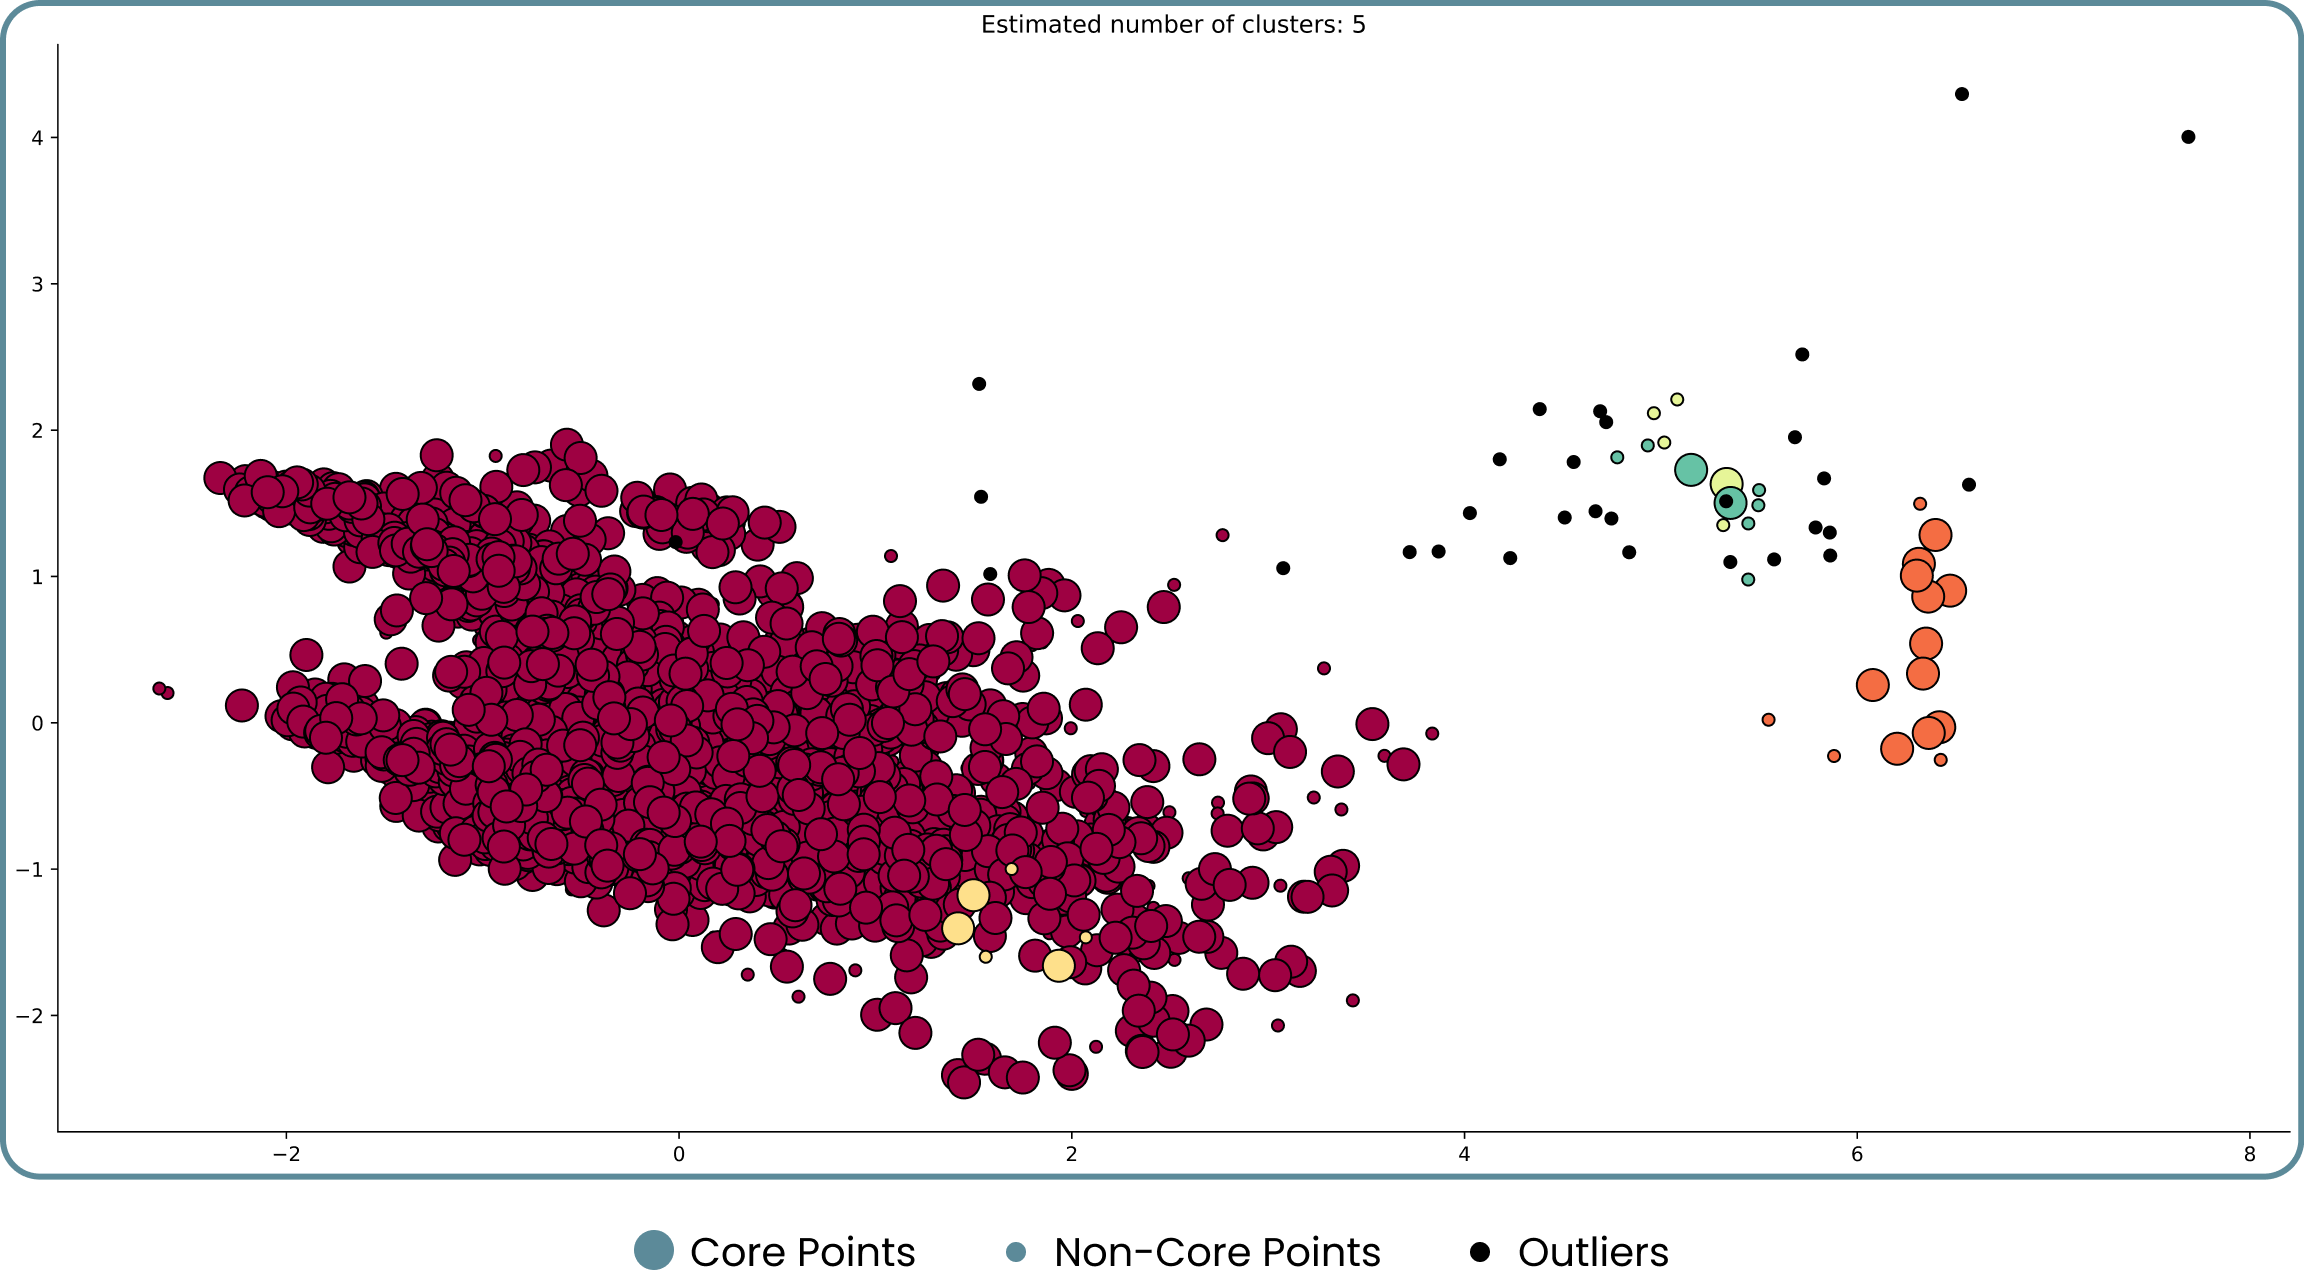
\includegraphics[width=13cm]{Images/3/clusters.png}
    \caption{Graphic representation of clusters in 2 components with PCA}
\end{figure}

Probably because these are \textit{dummy} dimensions, this depiction is not very meaningful to look at with the naked eye, but it does give insight into how the DBSCAN worked. In fact, the different colors with which the points are represented represent the different clusters generated. Instead, the size of the dot distinguishes \textbf{core points} from \textbf{non-core points}. Finally, the small black dots represent the \textbf{outliers} highlighted by the algorithm.


\subsection{Features importance}
\label{sec:testing-importance}

As described in the \ref{sec:importance} section, a key step was to analyze the feature importance for each model after DBSCAN implementation thanks to logistic regression.

\begin{figure}[H]
    \centering
    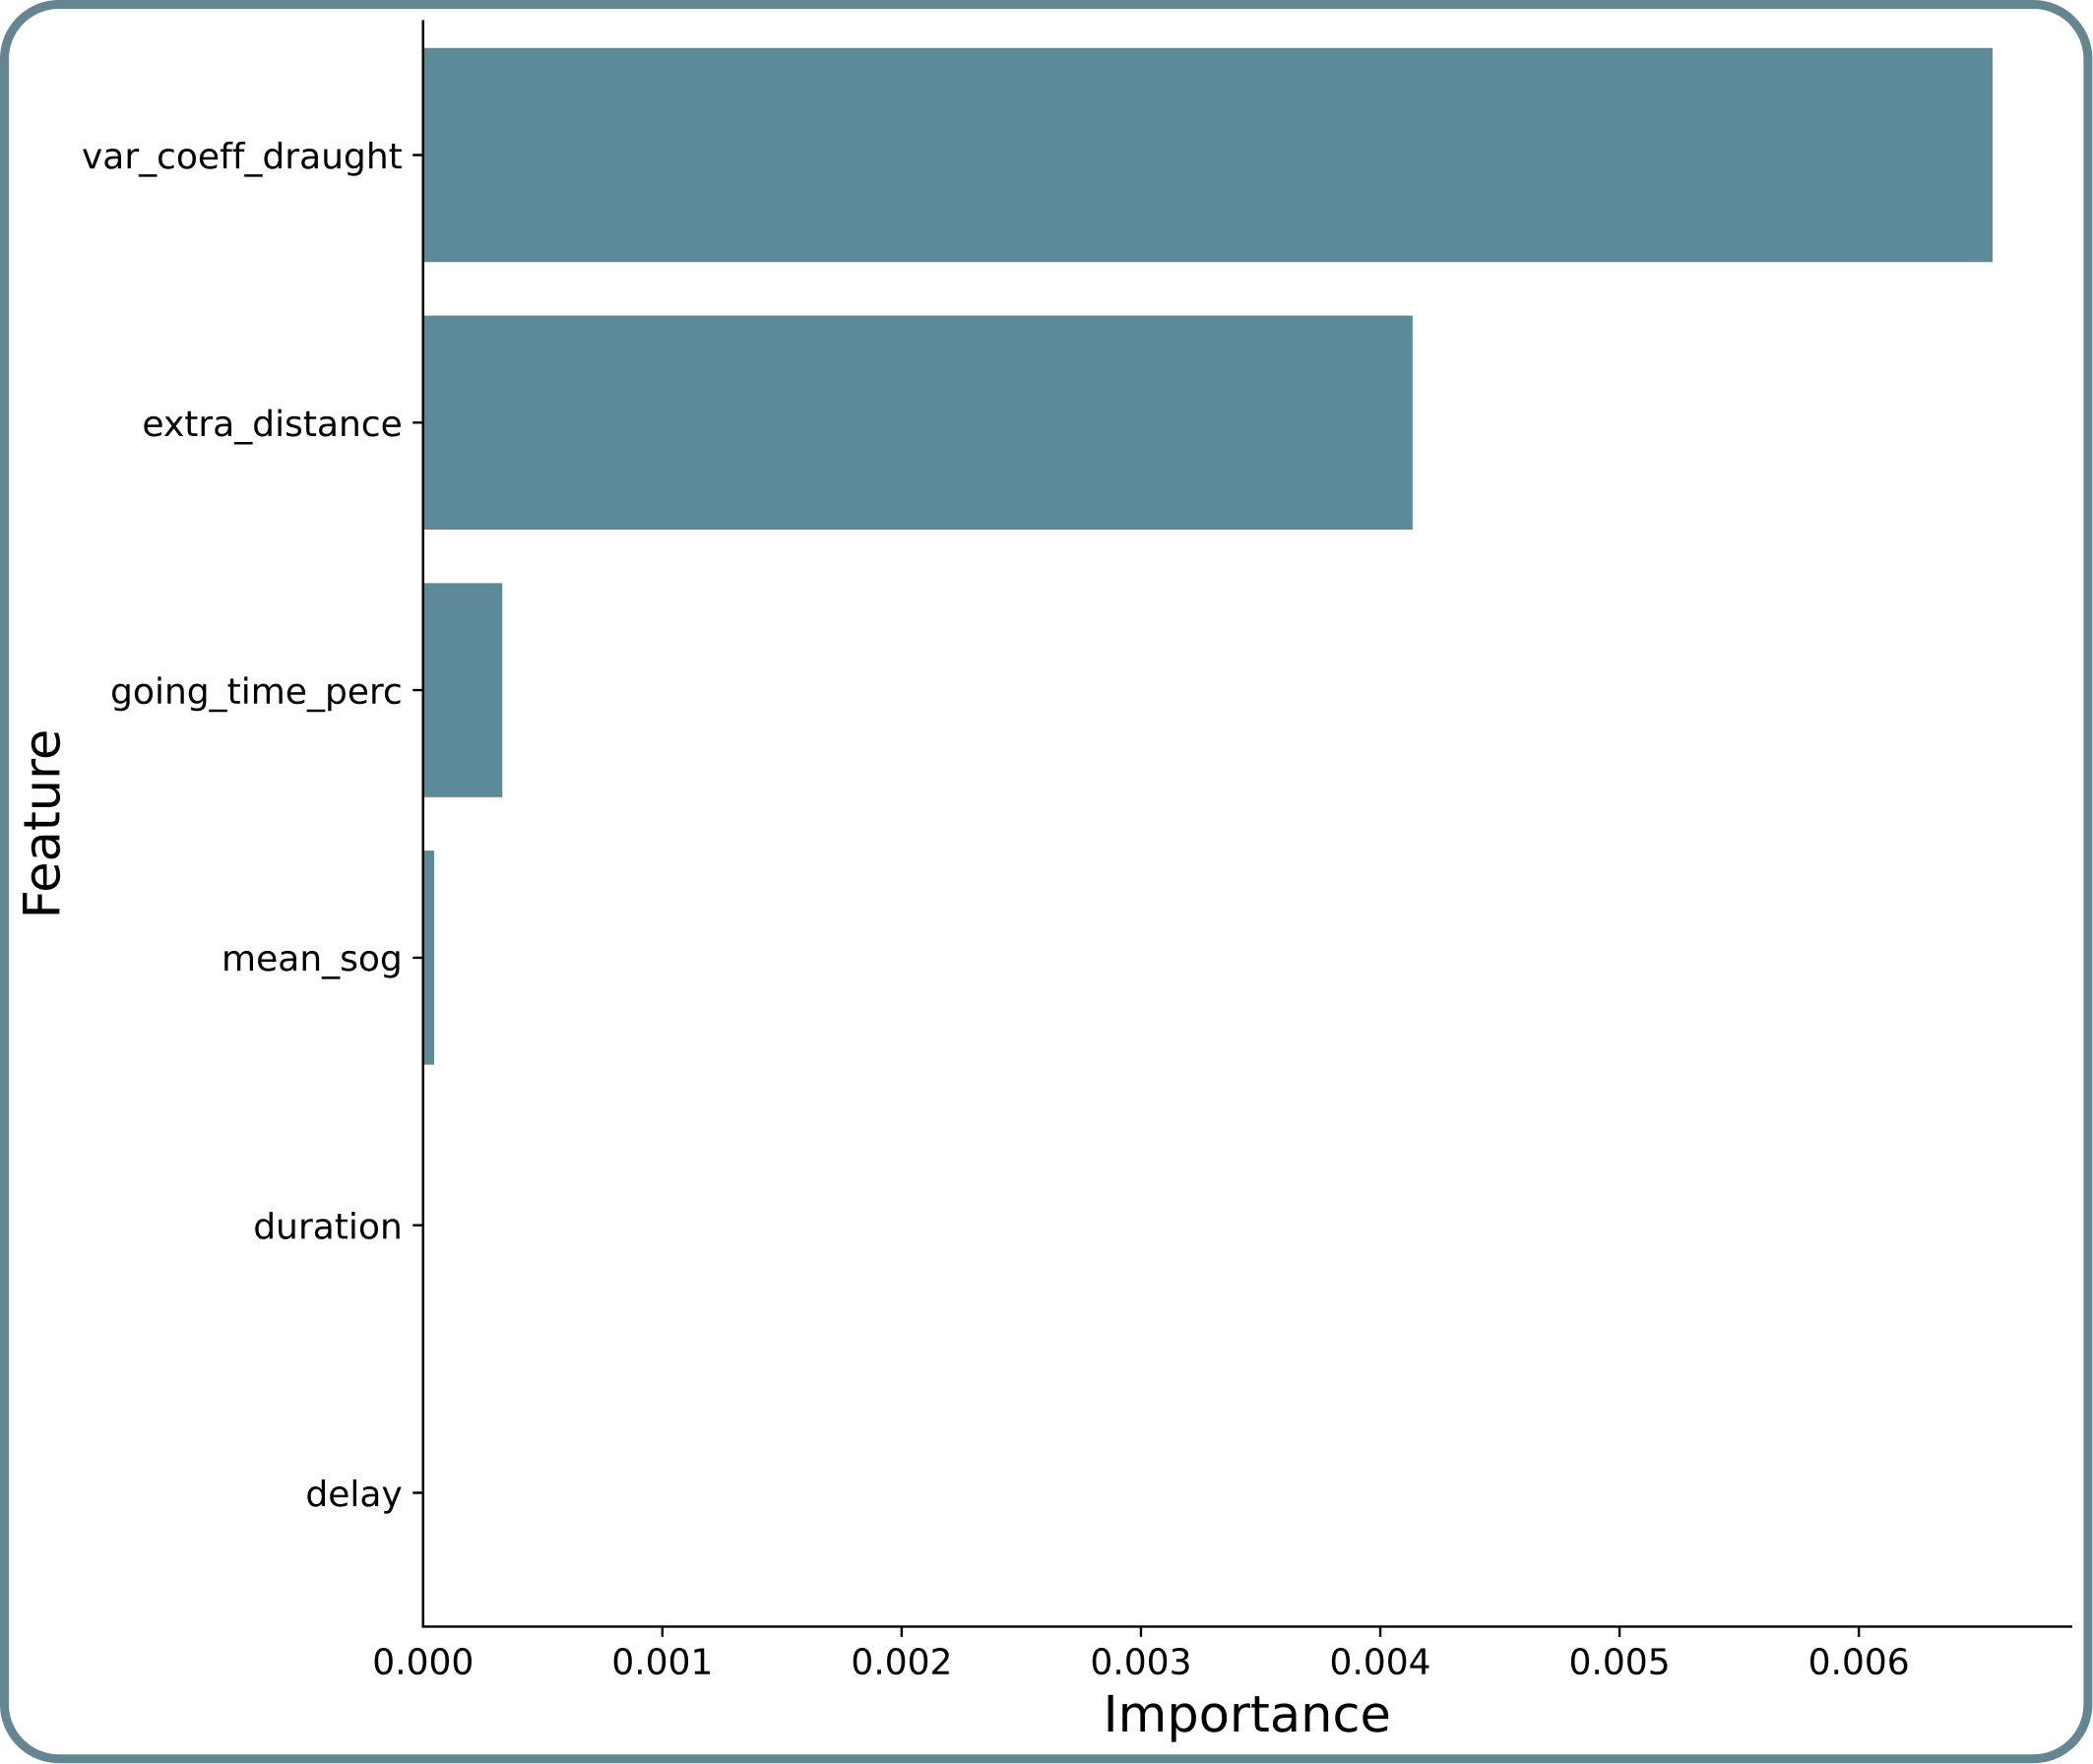
\includegraphics[width=13cm]{Images/3/importance.png}
    \caption{Feature importance classification for Cluster \#1}
\end{figure}

By having a graph like this for each cluster, it was possible to understand overall which features are most important for the purpose of classifying outliers.

\clearpage
\subsection{Anomaly 1 - Extra distance}
\label{sec:anomaly-1}

\begin{itemize}
\item Model Accuracy: \textbf{0.9189} \textcolor{green}{> 0.8}
\item T-test p value: \textbf{3.32e-03} \textcolor{green}{< 0.05}
\item Average Value for outliers: \textbf{196km}
\item Average Value for non outliers: \textbf{67.24km}
\end{itemize}

The anomaly related to the feature \textbf{extra distance} occupies the top position in most rankings of feature importance rankings of the resulting models.

Of course, routes with land points within the route were not considered in the evaluation of this anomaly, since for this type of trip it is quite normal to have an effective length much greater than the ideal length.

\begin{lstlisting}[language=Python]
extra_distance = ideal_distance - actual_distance
\end{lstlisting}

The \textbf{ideal distance} measures the distance in kilometers as the crow flies between the departure point to the arrival point. 
    
The \textbf{actual distance} measures the actual kilometers traveled by the ship during its trip. The calculation of this value is only possible by approximating the actual distance with the sum of the length of the different sections limited by the arrival of each message.

An abnormal number in this feature could mean that the voyage has experienced some disruptions or there may have been some unauthorized stops by the ship.

\begin{figure}[H]
    \centering
    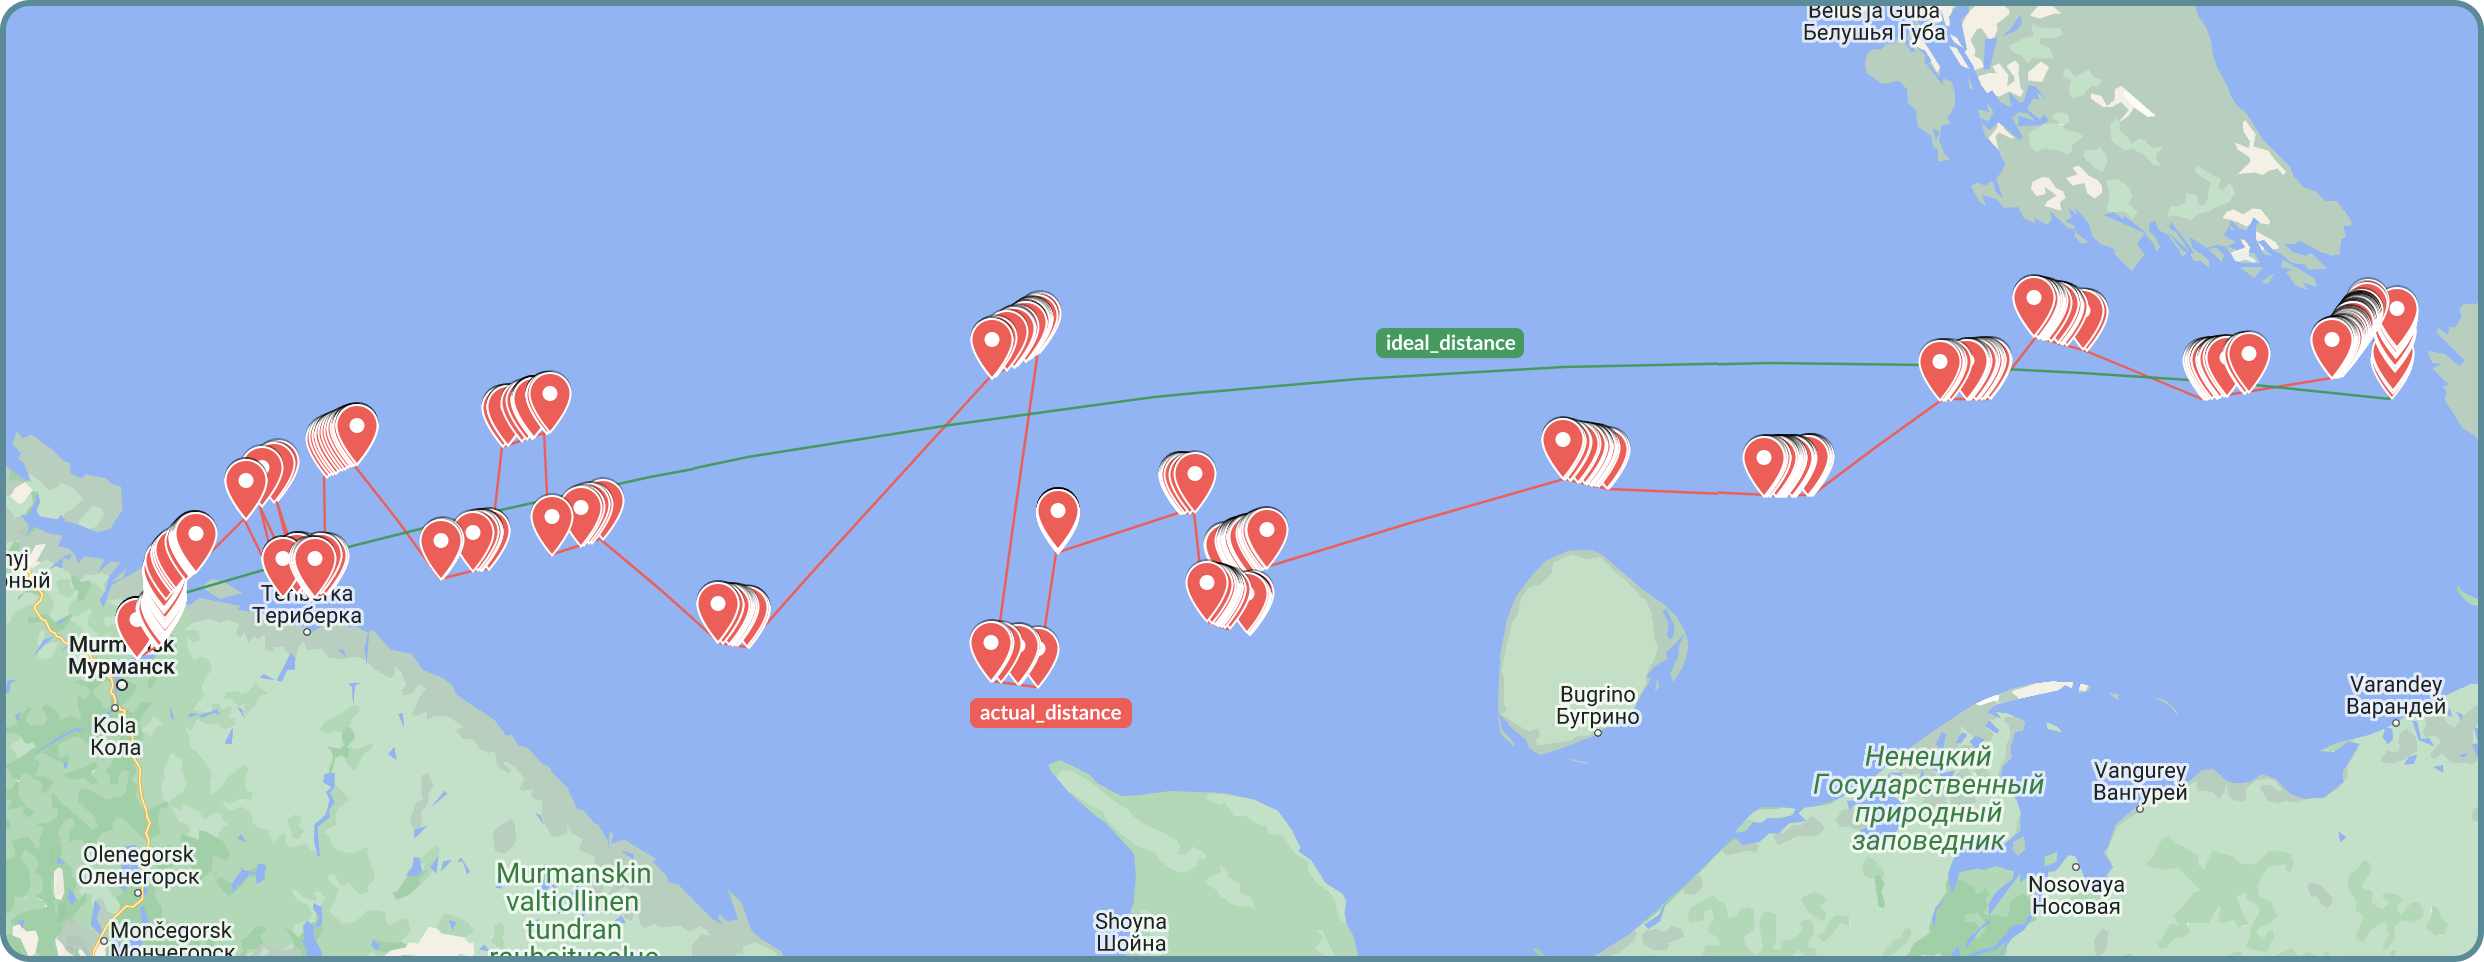
\includegraphics[width=16.5cm]{Images/3/anomaly-1.png}
    \caption{Vessel (MMSI 273397870) with a actual\_distance that differs greatly from the ideal\_distance.}
\end{figure}

\clearpage
\subsection{Anomaly 2 - Draught relative standard deviation}
\label{sec:anomaly-2}

\begin{itemize}
\item Model Accuracy: \textbf{0.9003} \textcolor{green}{> 0.8}
\item T-test p value: \textbf{3.32e-71} \textcolor{green}{< 0.05}
\item Average Value for outliers: \textbf{504.5}
\item Average Value for non outliers: \textbf{0.9957}
\end{itemize}

As explained in the appendix \ref{app:data-description} the draught of a vessel measures the maximum depth of any part of the vessel respect of the waterline, in meters. It might be considered a trivial measurement, but in maritime literature this value is used as a proxy for the weight of the ship's cargo.
\\
Since the dataset had different types of seagoing vessels with different sizes, a relative statistical measure indicating the level of draught variation during the voyage was computed, but relative to its own average.

\begin{lstlisting}[language=Python]
    var_coeff_draught = draught_arr.std() / draught_arr.mean() * 100
\end{lstlisting} 


\begin{figure}[H]
    \centering
    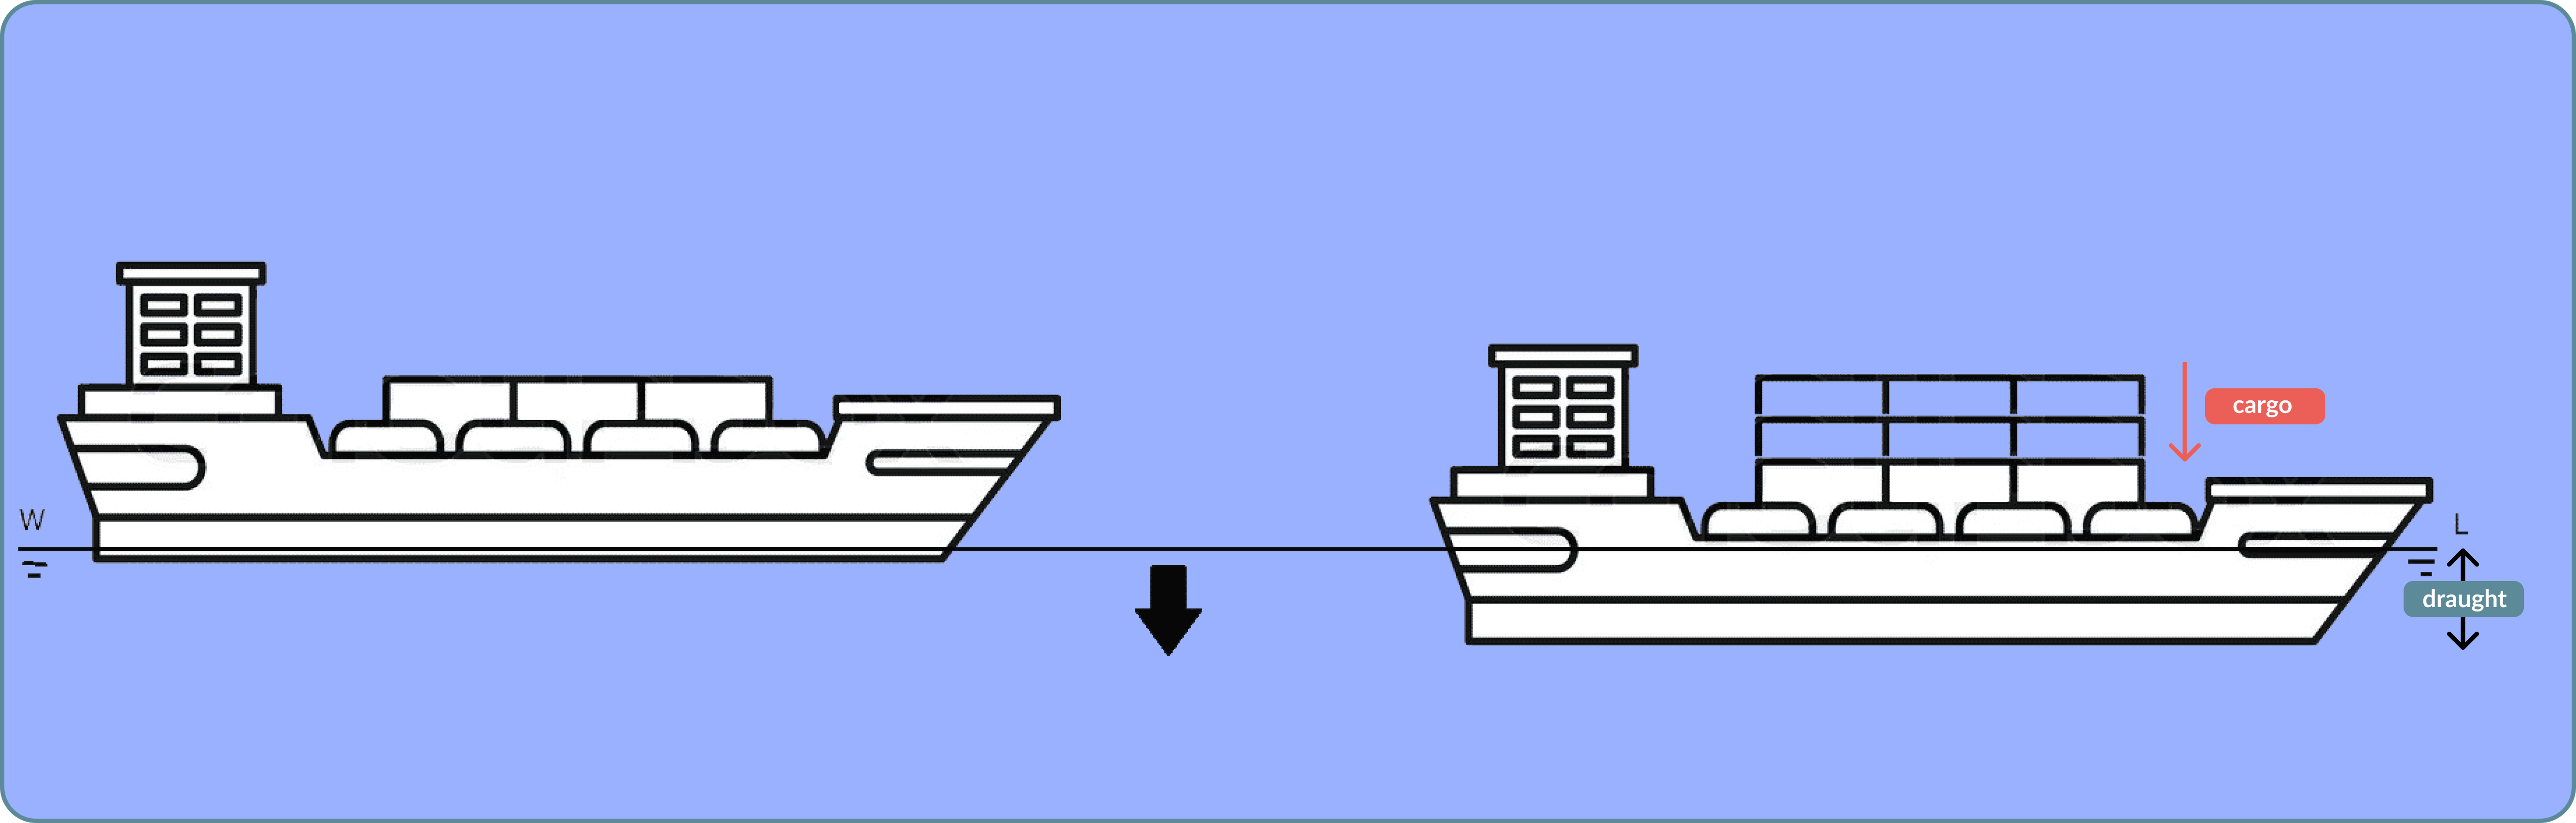
\includegraphics[width=16.5cm]{Images/3/anomaly-2.png}
    \caption{Draught value as proxy of cargo weight.}
\end{figure}

A high value of this feature means that the draught has fluctuated significantly during the distance travelled, and thus a fault may have occurred, or that the ship has unexpectedly varied the weight of its cargo. Further manual and individual analysis could be performed with information not included in the AIS to find out if the cargo is an illicit cargo.

\clearpage
\subsection{Anomaly 3 - Underway using engine percentage}
\label{sec:anomaly-3}

\\

\begin{itemize}
\item Model Accuracy: \textbf{0.8649} \textcolor{green}{> 0.8}
\item T-test p value: \textbf{4.71e-05} \textcolor{green}{< 0.05}
\item Average Value for outliers: \textbf{58.15}
\item Average Value for non outliers: \textbf{97.17}
\end{itemize}
\\

Each AIS message also contained ship status information. The most common value of this field is '\textit{Underway using engine}'. With this information it was possible to calculate an approximation that measures how much time the ship spent in this status.
According to this anomaly, however, there are voyages that have a lower percentage of time spent in this state than usual, as can be seen from the difference between the average value for outliers versus non-outliers.
\\
\begin{lstlisting}[language=Python]
    going_time_perc = going_time / duration * 100
\end{lstlisting} 
\\
By graphically depicting these trips on a map, one can see standoff points where the ship stopped for a substantial amount of time. Again, by cross-referencing additional information, the precise reason can be determined.


\begin{figure}[H]
    \centering
    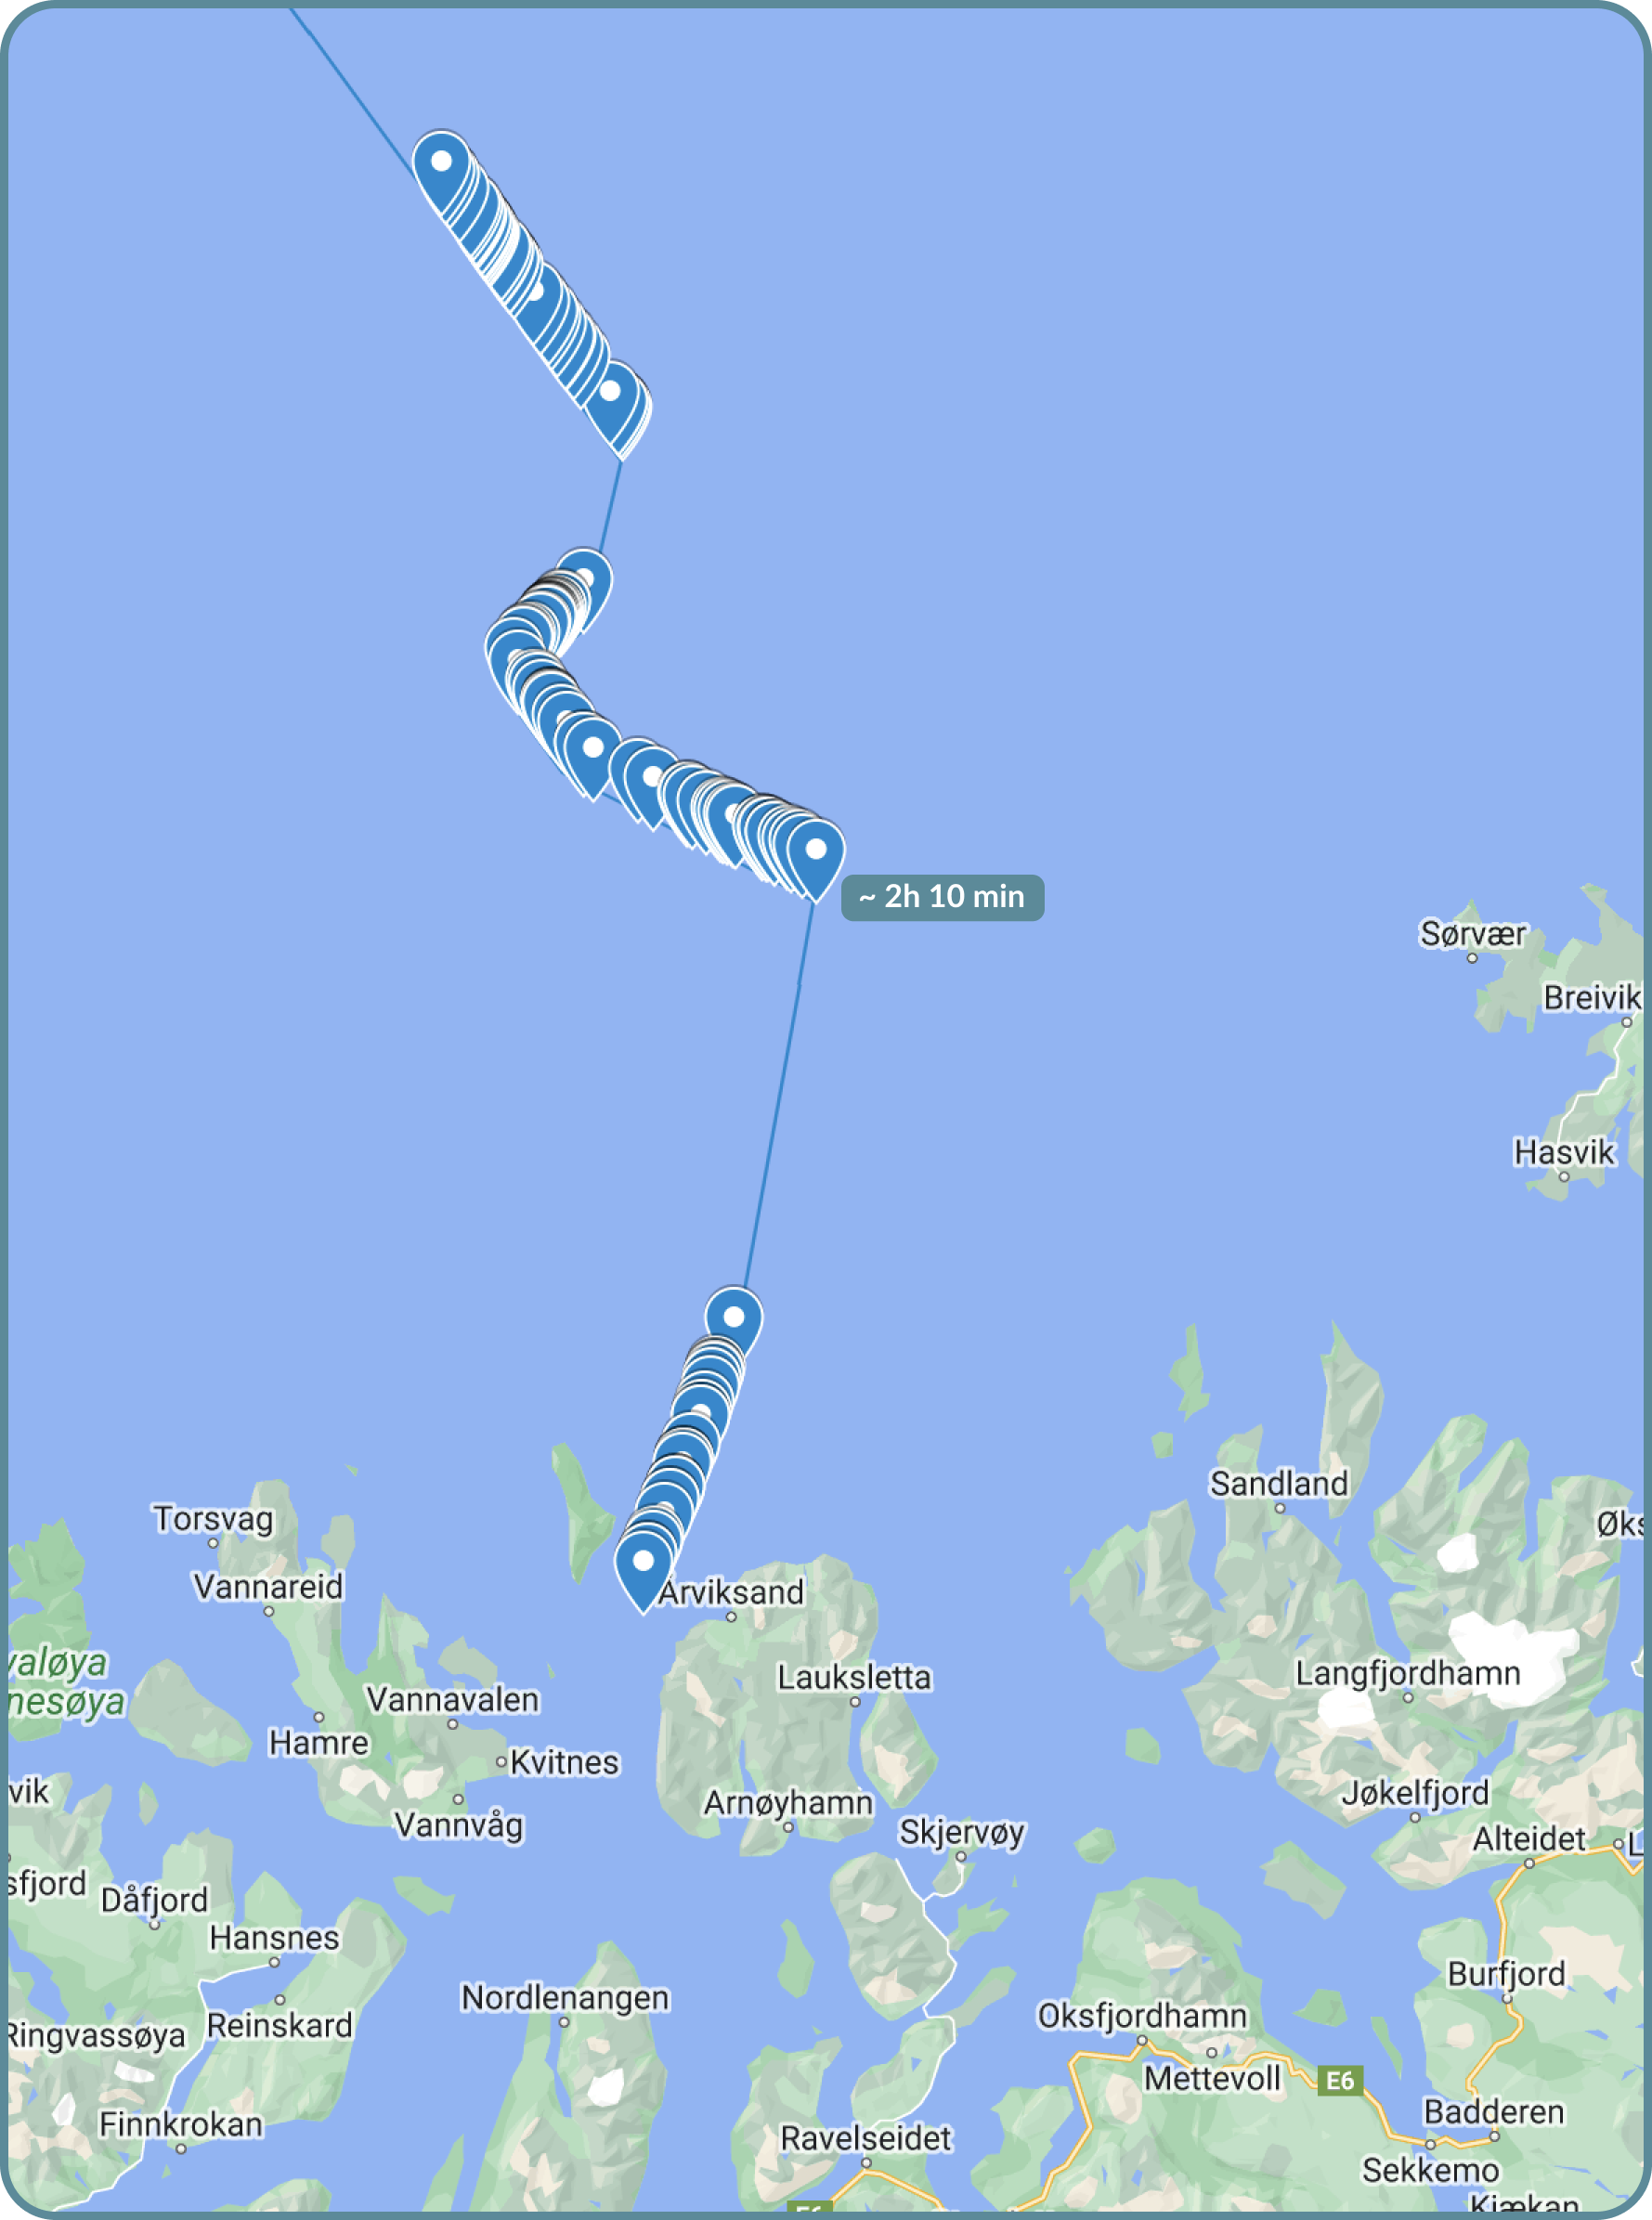
\includegraphics[width=12cm]{Images/3/anomaly-3.png}
    \caption{Vessel (MMSI 273397870) with anomal going time stall point.}
\end{figure}
